\section{Results} %{{{
\begin{figure}[t]
  \centering
  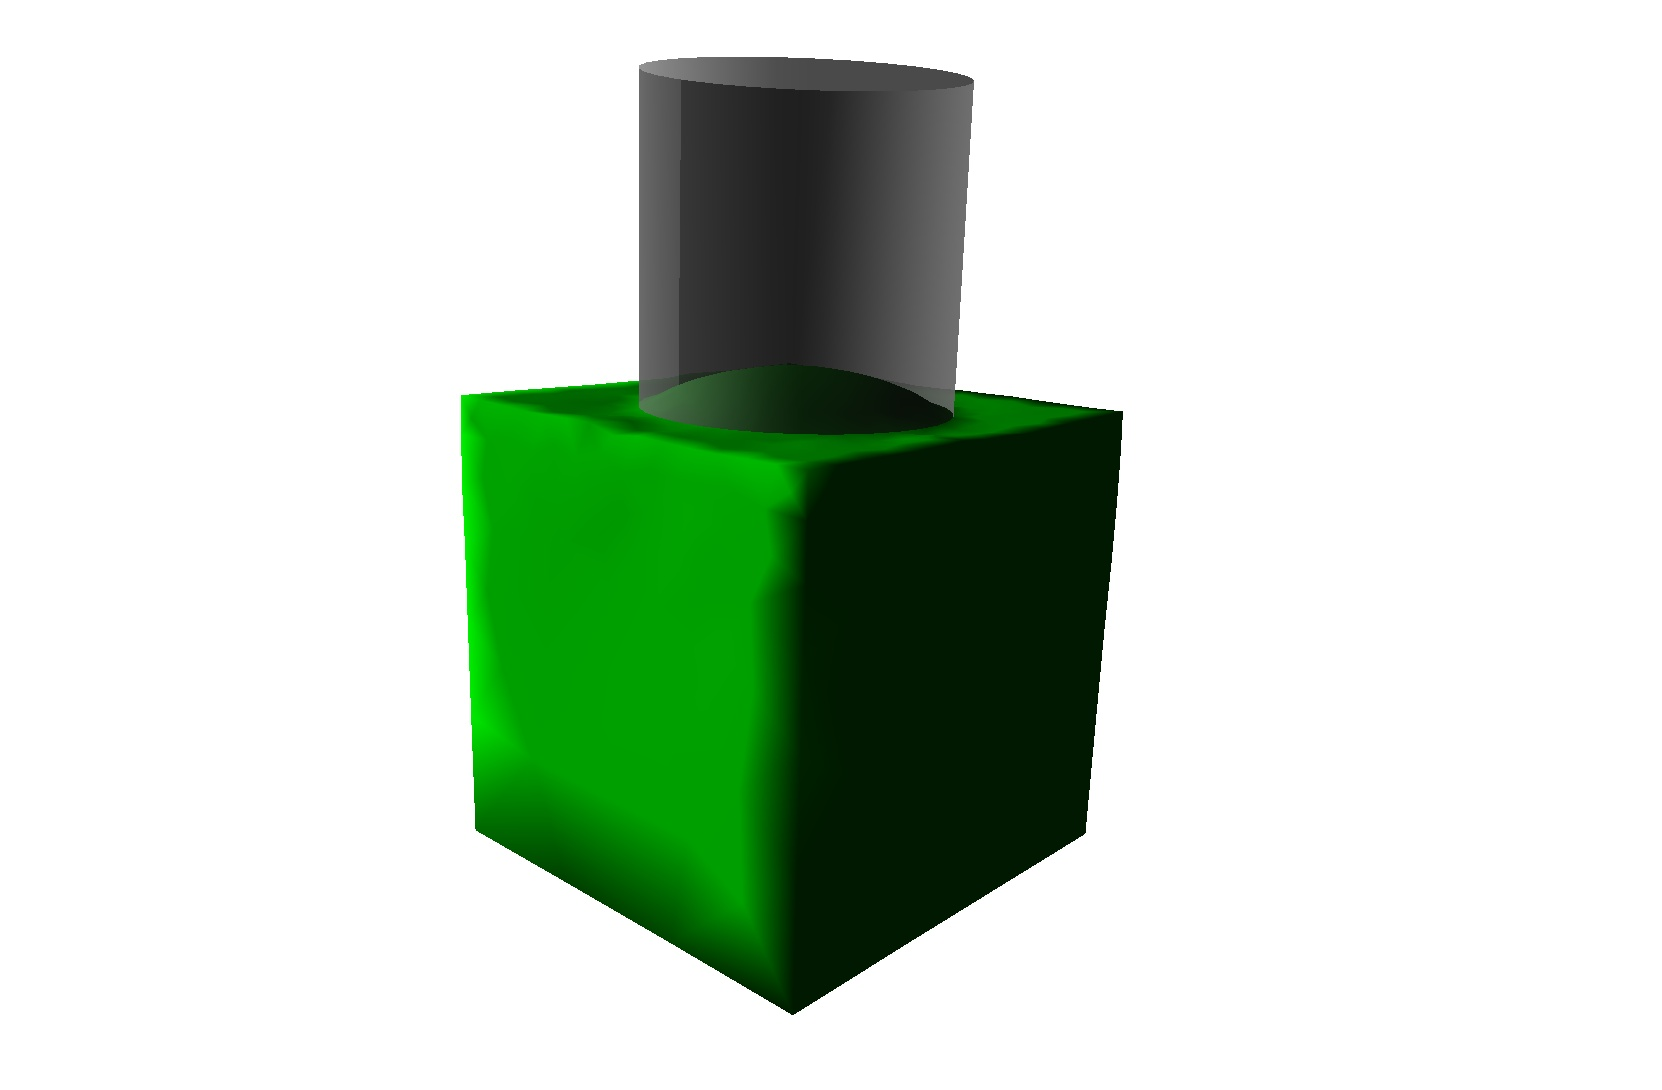
\includegraphics[height=3.5cm]{figures/aspirationScreenshot.jpg}
  \caption{\label{fig-aspiration1} The SOFA simulation scene of the aspiration test.}
\end{figure}
\subsection{Aspiration Test}
% As the first step, we evaluate the influence of the Glisson's capsule on the mechanical response of the tissue during
% the aspiration test. 
In~\cite{Hollenstein2006} an \emph{aspiration test} is presented to quantify the local influence of the Glisson's on tissue behaviour.
The aspiration device consists of a tube having 1\,cm in diameter and allows to
control the pressure inside the tube. The test is performed by
attaching the tube to the tissue and measuring the tissue response. We
set up a simulation in SOFA to reproduce the experiment (see
Fig.~\ref{fig-aspiration1}): we meshed a 15$\times$15$\times$15\,mm$^3$ 
cube representing the tissue resulting in 2648 tetrahedra. Then we attached a 1\,cm tube 
and applied a pressure of 3\,kPa inside the tube. The contacts between the tube and tissue sample were modeled using 
an approach based on non-linear complementarity problem presented in~\cite{Duriez2006b} which provides a solution for 
the Signorini's problem while taking into account friction between the objects.
% objects

According to~\cite{Hollenstein2006} the influence of the capsule is significant: modeling 
only the parenchyma without considering the membrane results in overestimation of the deformation by a factor of 2 to 3. 
In order to verify this observation, we performed a simulation using capsule parameters measured experimentally on 
ex-vivo pig liver~\cite{Umale2011}: Young's modulus of the membrane was set to $E_c$=8.22\,MPa and thickness was
$t_c$=20\,$\mu$m. 
Since the values for parenchyma elasticity reported in the literature vary significantly being usually reported between 2\,kPa to 5\,kPa, 
we employed a value $E_p$=3.5\,kPa for the Young's modulus of the parenchyma. 

\begin{figure}[t]
  \centering
  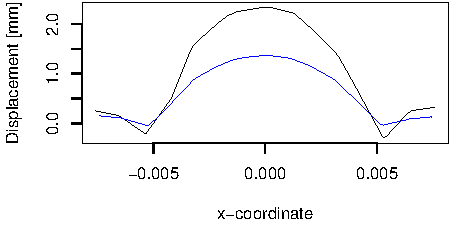
\includegraphics[width=7cm]{figures/displacementProfile.pdf}
  \caption{\label{fig-aspiration2} Displacement profile of the cube in the
  aspiration test with (blue) and without (black) the capsule.}
\end{figure}

\begin{figure}
  \centering
  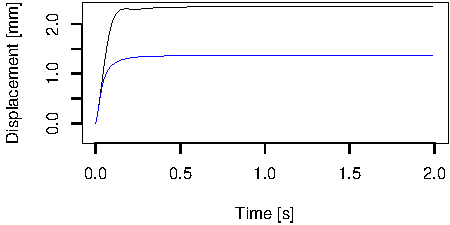
\includegraphics[height=3.5cm]{figures/displacementEvolution.pdf}
  \caption{\label{fig-aspiration3} Evolution of the displacement at the center
  in time for test with (blue) and without (black) the capsule.}
\end{figure}

In Fig.~\ref{fig-aspiration2} the profiles of cuts in the middle of the
test cube are presented showing significantly larger deformation in the model without capsule assuming that the same negative pressure was applied 
on the tissue surface inside the tube. Moreover, it can be observed that the deformation without capsule is overestimated by a factor 
close to 2, which is in perfect agreement with the results reported in~\cite{Hollenstein2006}.
Fig.~\ref{fig-aspiration3} presents the evolution of displacement in time at central node on the cube surface showing clear the effect of increased combined stiffness.

Further, we employed the simulation to reproduce the displacements values obtained via simulation in~\cite{Hollenstein2006,Nava2008}.
Whereas the simulation in the referenced work was done on a mesh composed of tetrahedral elements for both the parenchyma 
and the capsule, we employ the membrane CST elements.

Since the Young's moduli of neither parenchyma ($E_p$) nor capsule ($E_c$) were specified exactly, we obtained both as follows: first, 
we performed a set of simulations without the capsule for different values of $E_p$: the value that provided a good match 
with reported displacements was $E_p$=30\,kPa. 
Then, we fixed the thickness of the capsule to be $t$=93\,$\mu$m (reported as the average value in the paper) and 
using $E_p$=30\,kPa, we ran the simulation repeatedly using the model with the capsule. In each simulation we 
used different value $E_c$ of the Young's modulus for the capsule in order to minimize the displacement error w.r.t. the 
reported values. The minimal value of error (not exceeding 1\%) was obtained for $E_c$=3\,MPa. This 
value lies in the range of capsule elasticity coefficients reported by experimental measurements.

% % % %Moreover, we are able to reproduce
% % % %the measurements presented in~\cite{Hollenstein2006,Nava2008} with less than 1\% error.
% % % %We do not model the time-dependent behaviour though.
% % % %In this simulation we prescribe the the internal pressure of 30\,kPa. The other
% % % %parameters of the model were obtained like this: First we fix the stiffness of
% % % %parenchyma to $E_p$=30\,kPa to match the scenerio without capsule. Then,
% % % %assuming the thickness $t$=93\,$\mu$m of the capsule (reported as average in
% % % %the paper) we run several simulations with different capsule stiffness $E_c$.
% % % %We have found the lowest error is when $E_c$=3\,MPa. All the stiffness
% % % %parameters lie within the ranges measured in the paper.
% % % 
% % % %In this case the simulation was performed with the pressure of 30\,kPa and with
% % % %the following elastic parameters: $E_p$=30\,kPa for parenchyma and $E_c$=3\,MPa
% % % %and $t$=93\,$\mu$m for capsule.
% % % %All the values lie within the measurements
% % % %specified in the paper. \TG{add figure like Fig. 2?}
% % % 
% % % %The influence of the capsule on local level has been published in literature
% % % %before. However, to our knowledge it's influence on global scale deformation
% % % %has not been studied yet. We believe that the capsule has non-negligible impact
% % % %also on global level. 

% In the scenario presented in this paper, we focus on local influence of the capsule.
% Nevertheless, it is possible to employ the actual model to demonstrate the global 
% impact of the capsule and to further validate the accuracy of such a complete model w.r.t. experimental measures. 
% Detailed description of such validation is however beyond the scope of this paper. 
% In spite of this we would like to emphasize that we have already integrated the
% capsule model with vascularized liver model described in~\cite{Peterlik2012}. 
% Adding the capsule did not affect the
% performance significantly: a visual refresh rate exceeding 25\,FPS was achieved on a
% PC with CPU Intel i7 running at 3.00 GHz.
% This suggests that the proposed technique is compatible with real-time simulation of whole
% organ while modeling the local properties accurately.

%In our future work we need to validate the model in the
%context of global and local deformations. This task is challenging because
%comparing in vivo measurements with the simulation is difficult due to complex
%boundary conditions. 
%\TG{ex-vivo: no information abou vessels; phantoms: cannot model capsule}

%}}}

\begin{figure}[b]
  \centering
  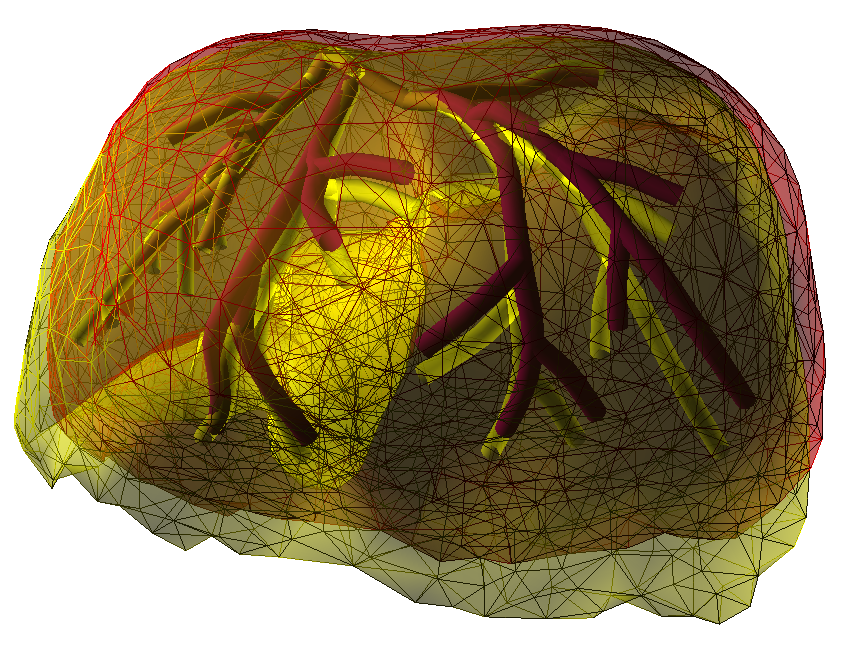
\includegraphics[height=7cm]{figures/modelUnderGravity.png}
  \caption{Liver under gravity with (red) and without (yellow) capsule}
  \label{f:gravity}
\end{figure}


\subsection{Global Deformation of Complete Model}
The complete model was constructed using contrast-enhanced CT data acquired on a female pig.
The liver and hepatic vein were segmented using semi-automatic methods available in ITKSnap~\footnote{www.itksnap.org}.
A tetrahedral mesh was obtained from the segmented maps using CGAL~\footnote{www.cgal.org}.
The semi-automatic method presented in~\cite{Peterlik2012} was
then applied to the segmented map of the hepatic vein, resulting in linked-beam model.
Finally, the model of the Glisson's capsule was constructed using the surface elements extracted from the volume mesh.
%described in section~\ref{ss:capsuleModel} over the surface triangles extracted from the tetrahedral mesh.
The complete model composed of 4266 tetrahedra, 188 beams and 1284 triangles was 
used in simulation where external force representing the gravity was applied to the model,
resulting in large deformations mainly in the area of lobes. The refresh rate of 22\,FPS
was achieved on a desktop computer with Intel i7 CPU running at 3.4\,GHz and 8\,GB of memory.
The simulation with gravity was also used as a first demonstration of the global influence of the capsule.
In Fig.~\ref{f:gravity}a, the models with capsule (red) and without (yellow) are depicted after being
deformed due to the gravity, showing a significant difference between the two models.



